\documentclass[conference]{IEEEtran}
\IEEEoverridecommandlockouts
% The preceding line is only needed to identify funding in the first footnote. If that is unneeded, please comment it out.
\usepackage{amsmath,amsthm,amssymb} %modos matemáticos y  simbolos
\usepackage{latexsym,amsfonts} %simbolos matematicos
\usepackage{cancel} %hacer la linea que cancela las ecuaciones
\usepackage[spanish, es-noshorthands]{babel} %comandos en español y cambia el cuadro por la tabla
\decimalpoint %cambia las comas por puntos decimal
\usepackage[utf8]{inputenc} %caracteristicas del español
\usepackage{physics} %Simbolos fisicos
\usepackage{array} %mejores formatos de tabla
\parindent =0cm %sangria 
\usepackage{algorithmic}
\usepackage{graphicx}
\usepackage{textcomp}
\usepackage{xcolor}
\usepackage{mathtools} 
\usepackage[framemethod=TikZ]{mdframed}%Entornos talegas
\usepackage[colorlinks = true,
			linkcolor = blue,
			citecolor = black,
			urlcolor = blue]{hyperref}%formato de los links y URL's
\usepackage{multicol} %varias columnas
\usepackage{enumerate} %enumeraciones
\usepackage{pgf,tikz,pgfplots} %documentos en formato tikz
\usepackage{mathrsfs} %letras chingonas (transformada de laplace)
\usepackage{subfigure} %varias figuras seguidas
\usepackage{tabulary}
\usepackage{multirow} %ocupar varias filas en una tabla
\usepackage{fancybox} %recuadros talegas
\usepackage{float} %ubicar graficas
\usepackage{color}
\usepackage{comment}
\usepackage{stackrel}
\usepackage{calligra}
\usepackage{lipsum}
\usepackage{cite}
\pgfplotsset{compat=1.16} 

\newcommand{\R}{\mathbb{R}}
\newcommand{\Z}{\mathbb{Z}}
\newcommand{\Q}{\mathbb{Q}}
%%%%%%%%%%%%%%%%%%%%%%%%%%%%%%%%%%%%%%%%%%%%%%%%%%%%%%
\def\BibTeX{{\rm B\kern-.05em{\sc i\kern-.025em b}\kern-.08em
    T\kern-.1667em\lower.7ex\hbox{E}\kern-.125emX}}
\begin{document}

\title{Proyecto Genérico \\
{\footnotesize \scshape{Sistemas Dinámicos, Segundo Semestre 2023}}
}

\author{\IEEEauthorblockN{1\textsuperscript{st} Diego Sarceño Ramírez}
\IEEEauthorblockA{\textit{201900109} 
}
%\and
%\IEEEauthorblockN{2\textsuperscript{nd} Andrés Pérez}
%\IEEEauthorblockA{\textit{201704199}
%}
%\and
%\IEEEauthorblockN{3\textsuperscript{rd} Diego Sarceño Ramírez}
%\IEEEauthorblockA{\textit{201900109} \\
%}
}



\maketitle


\section{Capítulo 1}

\subsection{Problema 1.1}
Para $h(x) = rx(1-x)$ y $n = \{ 0,1,2,3,4,101,102,103,104 \}$.

\begin{enumerate}[a)]
	\item Con $r = 2$ y $x = 0.25$.
	\item Con $r = 2$ y $x = 0.2345$.
	\item Con $r = 3.1$ y $x = 0.25$.
	\item Con $r = 3.1$ y $x = 0.252345$.
	\item Con $r = 4$ y $x = 0.25$.
	\item Con $r = 4$ y $x = 0.2345$.
\end{enumerate}




\subsection{Problema 1.3}
Diagramas de Fase realizados en \textit{Mathematica}.

\begin{enumerate}[a)]
	\item $f(x) = x^{1/3}$.
		\begin{figure}[H]
			\centering
			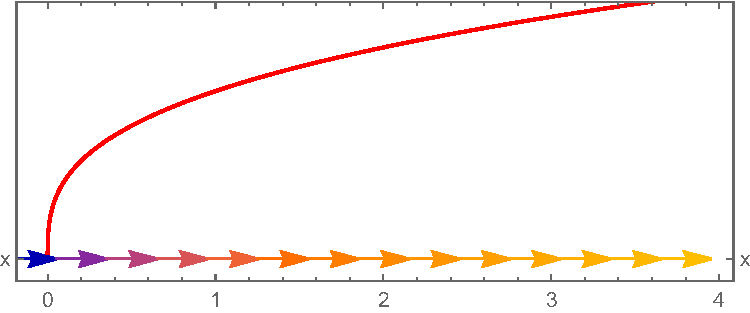
\includegraphics[scale=0.4]{./img/p1-3_a}
		\end{figure}
	\item $g(x) = 2\arctan{x}$.
		\begin{figure}[H]
			\centering
			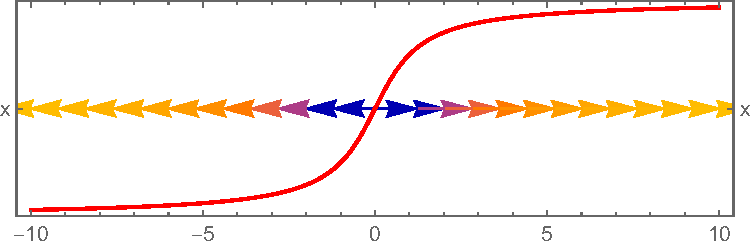
\includegraphics[scale=0.4]{./img/p1-3_b}
		\end{figure}
	\item $r(x) = 1/x$.
		\begin{figure}[H]
			\centering
			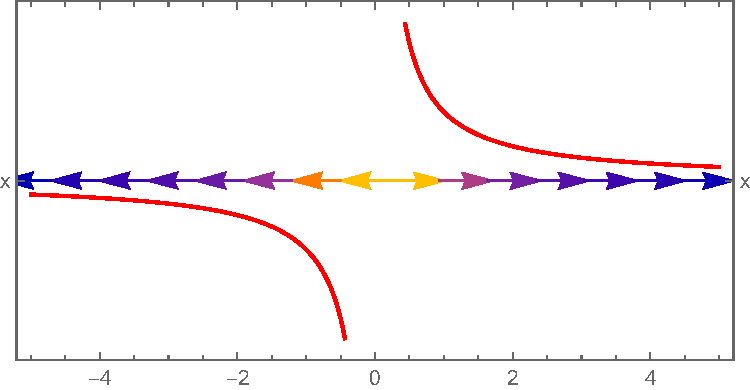
\includegraphics[scale=0.4]{./img/p1-3_c}
		\end{figure}
	\item $C(x) = \cos{x}$.
		\begin{figure}[H]
			\centering
			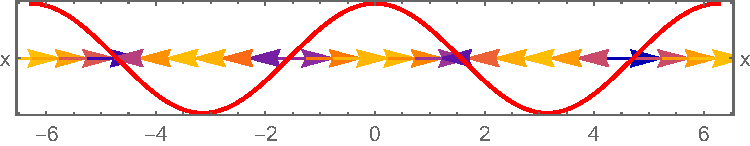
\includegraphics[scale=0.4]{./img/p1-3_d}
		\end{figure}
\end{enumerate}




\section{Capítulo 2}

\subsection{Problema 2.1}
\begin{enumerate}[a)]
	\item Viendo la gráfica de la función $f(x) = x^2$, es claro que $f([0,1]) \to [0,1]$.
		\begin{figure}[H]
			\centering
			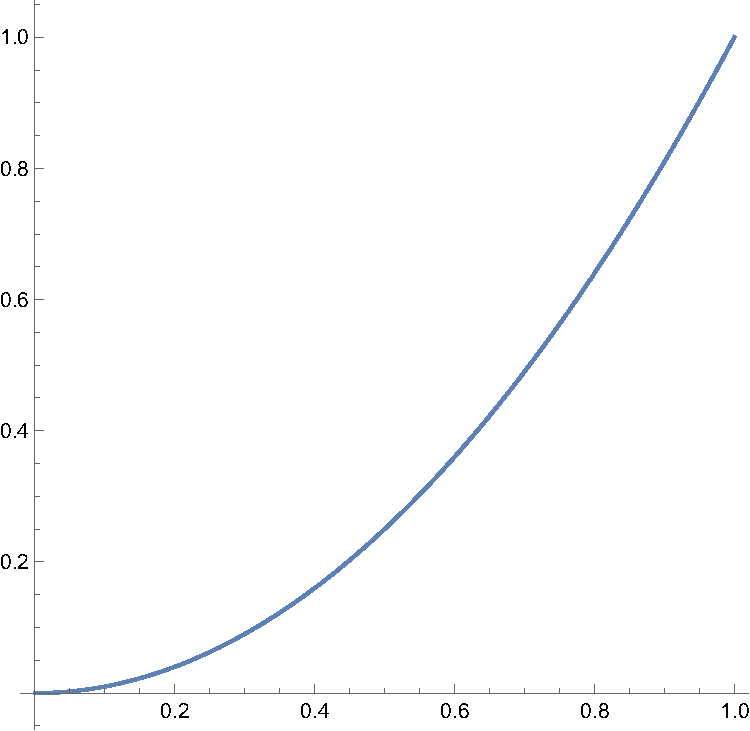
\includegraphics[scale=0.35]{./img/p2-1}
		\end{figure}
	\item Para el intervalo dado, la función $x^2$ es invertible, entonces $f^{-1}(x) = \sqrt{x}$, por lo que $f^{-1} (f([0,1])) = f(f^{-1}([0,1])) \to [0,1]$ al menos para el intervalo dado.
	\item Con $S(x) = \sin{x}$ se sabe que $S([0,\pi /2]) \to [0,1]$; por lo que $S^{-1} (x) = \arcsin(x) \, \Rightarrow \, S^{-1} (S([0,\pi /2])) \to [0,\pi /2]$.
\end{enumerate}




\subsection{Problema 2.4}
Suponga $f:[-1,1]\to [-1,1]$ está definido como $f(x) = \frac{1}{2} x$.
\begin{enumerate}[a)]
	\item Luego de valuar los puntos en el intervalo $[-1,1]$ estos se mapean en el intervalo $[-1/2,1/2]$.
	\item Para $f(f(x)) = \frac{1}{4} x$, sucede lo mismo que el inciso anterior, el rango es $[-1/4,1/4]$.
	\item Aplicando $f$ $n$ veces sobre sí misma, se tiene que $f^n (x) = \frac{1}{2^n} x$.
\end{enumerate}


\subsection{Problema 2.8 (Desigualdad del Triángulo)}
Sean $a,b \in \R$ y $-\abs{a,b} \leq a,b \leq \abs{a,b}$.

\begin{enumerate}[a)]
	\item Sumando las desigualdades dadas en el problema, se tiene $ -(\abs{a} + \abs{b}) \leq a+b \leq \abs{a} + \abs{b} $, lo que implica que $\abs{a + b} \leq \abs{a} + \abs{b}$.
	\item Reemplazamos $b$ por $-b$ en la desigualdad triangular, lo que nos da $\abs{a - b} \leq \abs{a} + \abs{-b} = \abs{a} + \abs{b}$.
	\item Restamos $\abs{b}$ en la desigualdad del inciso $b)$: $\abs{a} \geq \abs{a - b} - \abs{b}$. 
	\item Tomamos $a = a - b + b$ y aplicamos la desigualdad triangular $\abs{a} = \abs{(a - b) + b} \leq \abs{a - b} + \abs{b}$. Restamos $\abs{b}$ de ambos lados y: $\abs{a} - \abs{b} \leq \abs{a - b}$.
\end{enumerate}




\section{Capítulo 3}

\subsection{Problema 3.2}
Sea $x \in (a,b)$, se cumple que $a < x < b$, supongamos que $\varepsilon > 0$ es la distancia de $x$ al punto final más cercano de $(a,b)$ i.e. $\varepsilon = \min{x-a,b-x}$. Ahora sea $y\in B_\varepsilon (x) := \{ w\in \R \, | \, \abs{w-x} < \varepsilon \}$, entonces se cumple que $\abs{y-x} < \varepsilon$. Por la definición de $\varepsilon$ se tienen dos casos. \\

(CASO I.) $\varepsilon = x - a$,
	\begin{align*}
		\abs{y - x} &<  x - a \\
		-(x - a) < y &- x < x - a \\
		a < y &< 2x - a. 
	\end{align*}
(CASO II.) $\varepsilon = b - x$,
	\begin{align*}
		\abs{y - x} &<  b - x \\
		-(b - x) < y &- x < b - x \\
		2x - b < y &< b. 
	\end{align*}
Esto nos dice claramente que $a < y < b$, por ende $y\in (a,b)$. De esta forma, $B_\varepsilon (x) \subseteq (a,b)$, lo que implica que $(a,b)$ es un conjunto abierto.


\subsection{Problema 3.3}
La demostración es muy parecida a la realizada en el problema anterior, solo que esta vez la siguiente desigualdad $\abs{x - y} \leq \varepsilon \leq \abs{x - a}$. Por el mismo procedimiento del problema anterior, es claro que $a \leq y \leq 2x - a$ y $2x - b \leq y \leq b$. Por lo que $a \leq y \leq b$, lo que implica que la bola cerrada con radio $\varepsilon$ y radio $x$ pertenece al intervalo $[a,b]$, por lo que es un conjunto cerrado.


\subsection{Problema 3.5}
Si tomamos un número $q\in \Q$ y $r>0$, considerando un intervalo abierto $(q - r,q + r)$, este intervalo contendrá números irracionales, lo que implica que los números racionales no son un conjunto abierto.



\section{Capítulo 4}

\subsection{Problema 4.3}
Para $h(x) = 4x(1-x)$, se tiene la siguiente gráfica

\begin{figure}[H]
	\centering
	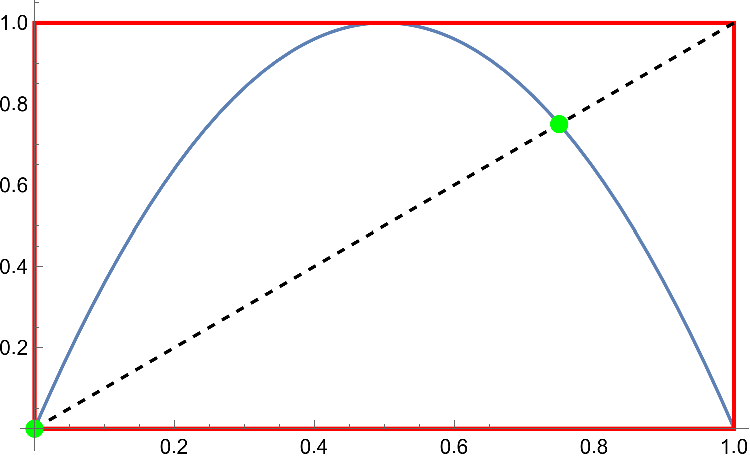
\includegraphics[scale=0.4]{./img/p4-3}
\end{figure}

\begin{table}[H]
	\centering
	\begin{tabular}{cc}
		Iteración 1 & $(9/16,27/64)$ \\
		Iteración 2 & $(3/4,9/16)$ \\
		Iteración 3 & $(3/4,3/4)$.
	\end{tabular}
\end{table}



\subsection{Problema 4.5}
Para $h(x) = 3.2x(1-x)$, se tiene puntos fijos en $x = 0$ y $x = 0.6875$ (luego de resolver la ecuación $3.2x(1-x) = x$), lo que demuestra que los puntos fijos están en el intervalo $[0,1]$.

\begin{figure}[H]
	\centering
	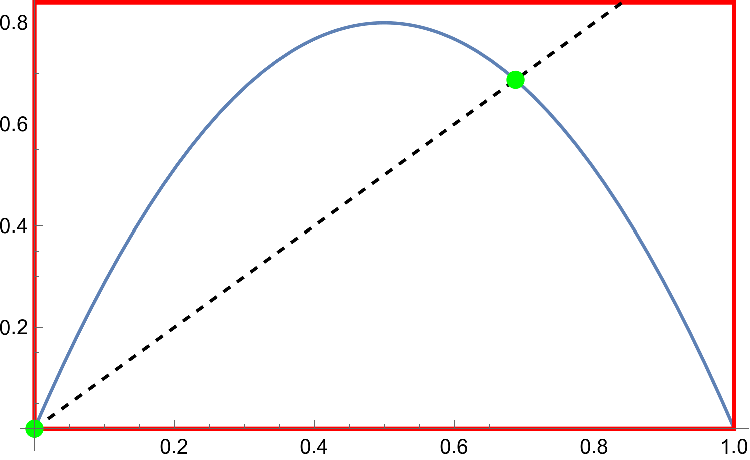
\includegraphics[scale=0.4]{./img/p4-5}
\end{figure}


\subsection{Problema 4.10}
Restringiendo el quinto polinomio de Legendre\footnote{$P_5 (x) = \frac{1}{2^5 5!} \dv[5]{x} [(x^2 - 1)^5] = \frac{1}{8} (63x^5 - 70x^3 + 15x)$.} a números positivos, se tiene

\begin{figure}[H]
	\centering
	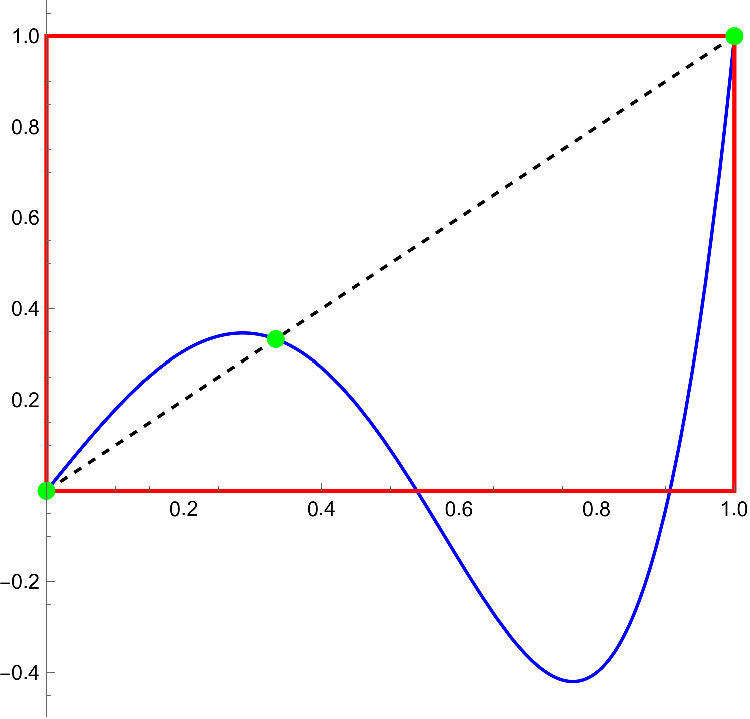
\includegraphics[scale=0.4]{./img/p4-10}
\end{figure}

Los puntos fijos estan en $x = 0,1/3,1$.





\section{Capítulo 5}

\subsection{Problema 5.3}









\section{Capítulo 6}

\subsection{Problema 6.1}
Encontramos los puntos fijos y si son atractores, repulsores, nodos o no están definidos.

\begin{enumerate}[a)]
	\item Para $f(x) = -x^3$, con puntos fijos reales $x = 0$ el cual es un nodo, ya que al valuar por derecha y por izquierda se tiene comportamiento atractor y repulsor.
	\item Para $f(x) = x^3 - x$, con puntos fijos en $x = \pm \sqrt{2}$ los cuales son repulsores y $x = 0$ el cuál es atractor.
	\item Para $f(x) = -x^3 - x$, con puntos fijos reales en $x = 0$ el cual es atractor.
	\item Para $f(x) = e^{x-1}$, con puntos fijos en $x = 1$ y dado el comportamiento alrededor de dicho punto se concluye que es un nodo.
	\item Para $f(x) = e^{-x}$, con punto fijo en $x = 0.567143$ el cual es un atractor.
	\item Para $f(x) = \sin{x}$, con puntos fijos en $x = 0$ el cual no está definido algebraicamente, pero realizando el gráfico es claro que es atractor.
	\item Para $f(x) = -x^{1/3}$, con punto fijo real en $x = 0$ el cual es atractor por la derecha.
	\item Para $f(x) = -\frac{4}{\pi} \arctan{x}$, con punto fijo en $x = 0$ el cual es atractor.
\end{enumerate}

Para ver los cálculos, revisar el notebook/pdf de mathematica.





\section{Capítulo 7}

\subsection{Problema 7.2}
Tomando $h_r (x) = rx(1-x)$.
\begin{enumerate}[a)]
	\item Resolviendo la ecuación $rx(1-x) - x = 0$ se tienen raíces $r = 0$ y $\frac{r-1}{r}$. Utilizando \textit{mathematica} o 
		\begin{align*}
			-rx^2 + (r-1)x &= 0 \\
			\frac{-(r-1)\pm \sqrt((r-1)^2)}{-2r} &= x \\
			x = 0 \qquad &\, \qquad x = \frac{r-1}{r} 
		\end{align*}
	\item El punto fijo $x = 0$ es repulsor dado que $r$ es positivo siempre. Y $x = \frac{r-1}{r}$ es repulsor para $0 < r < 2$, indeterminado para $r = 2$ y atractor para $r > 2$.
\end{enumerate}





\section{Capítulo 11}

\subsection{Problema 11.3}
\begin{enumerate}[a)]
	\item Dada $d_3 (x,y) = (x - y)^2$ verificamos que se cumplan los 4 axiomas
		\begin{itemize}
			\item Es claramente semidefinido positivo dado que $r^2 > 0 \, \forall \, r\in \R$.
			\item Identidad de los Indescernibles. $(\Rightarrow)$ $d_3 (x,y) = (x - y)^2 = 0 \, \Rightarrow \, x = y$.
				$(\Leftarrow)$ $x = y$ entonces $d_3 (x,x) = (x - x)^2 = 0$. Lo que cumple la identidad.
			\item Simetría. $d_3 (x,y) = (x - y)^2 = (-1)^2 (y-x)^2 = d_3 (y,x)$.
			\item Desigualdad triangular. Expandiendo ambos lados para verificar si se cumple o no para cualesquiera $x,y,z$. $x^2 + z^2 - 2xz + z^2 + y^2 - 2yz \geq x^2 + y^2 - 2xy \qquad \rightarrow \qquad 2z^2 + 2xy \geq 2xz + 2yz$ lo que no es necesariamente cierto para cualesquiera $x,y,z$.
		\end{itemize}
		Lo que implica que $d_3 (x,y) = (x - y)^2$ no es una métrica.
	\item Para $d_4 (x,y) = \frac{\abs{x - y}}{1 + \abs{x - y}}$ las primeras 3 propiedades se cumplen claramente, dado que $\abs{x - y}$ es una metría en sí. Por ende, solo hace falta ver si cumple la desigualdad triangular, y reemplazando los valores aboslutos por $a,b,c$ para facilidad
		$$ \frac{a}{1+a} + \frac{b}{1+b} \geq \frac{c}{1+c} , $$
	expandiendo y reduciendo términos semejantes
		$$ a + b + 2ab + abc \geq c. $$
	Lo que claramente se cumple dado que $\abs{x-y}$ es una métrica y cumple la desigualdad triangular $a + b \geq c$, y dado que todos son positivos, la desigualdad se cumple. Lo que implica que $d_4 (x,y)$ es una métrica.
\end{enumerate}

\section{Capítulo 14}

\subsection{Problema 14.1}
Simplificando
\begin{enumerate}[a)]
	\item $(2-3i) + (-1-4i) = 1 - 7i$.
	\item $\frac{1}{2} i - (1+i) = -1 - \frac{1}{2} i$.
	\item $(2+i)(i) = -1 + 2i$.
	\item $(2+i)/i = 1 - 2i$.
	\item $(1-4i)(2+3i) = 2 - 8i + 3i + 12 = 14-5i$.
	\item $\frac{1-4i}{2+3i} = \frac{1-4i}{2+3i} \frac{2-3i}{2-3i} = \frac{-10-11i}{13} = -\frac{10}{13} - \frac{11}{13}i$.
\end{enumerate}

\subsection{Problema 14.2}
Encontrando módulo y argumento utilizando \texttt{AbsArg[]} (usamos mathematica por practicidad, para aprovechar la herramienta y por la simplicidad del problema)
\begin{enumerate}[a)]
	\item $1-4i\, \to \, (\sqrt{17},-75.9639^o)$.
	\item $\frac{1}{2} + \frac{3}{4} i \, \to \, \qty(\frac{\sqrt{13}}{4},56.1499^o)$.
	\item $2\, \to \, (2,0^o)$. 
\end{enumerate}

\subsection{Problema 14.3}
\begin{figure}[H]
	\centering
	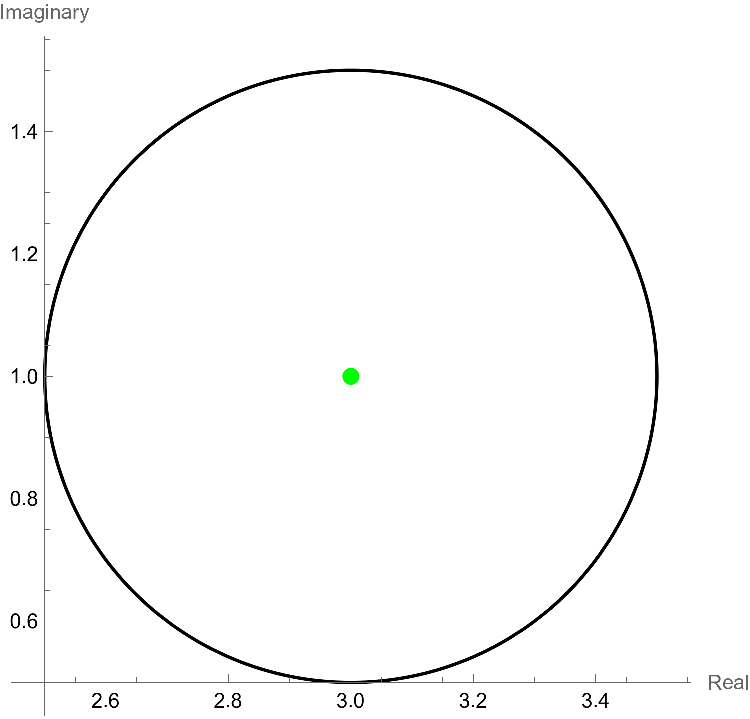
\includegraphics[scale=0.4]{./img/p14-3_a}
	\caption{Vecindad de radio $0.5$ del punto $3+i$.}
\end{figure}


\begin{figure}[H]
	\centering
	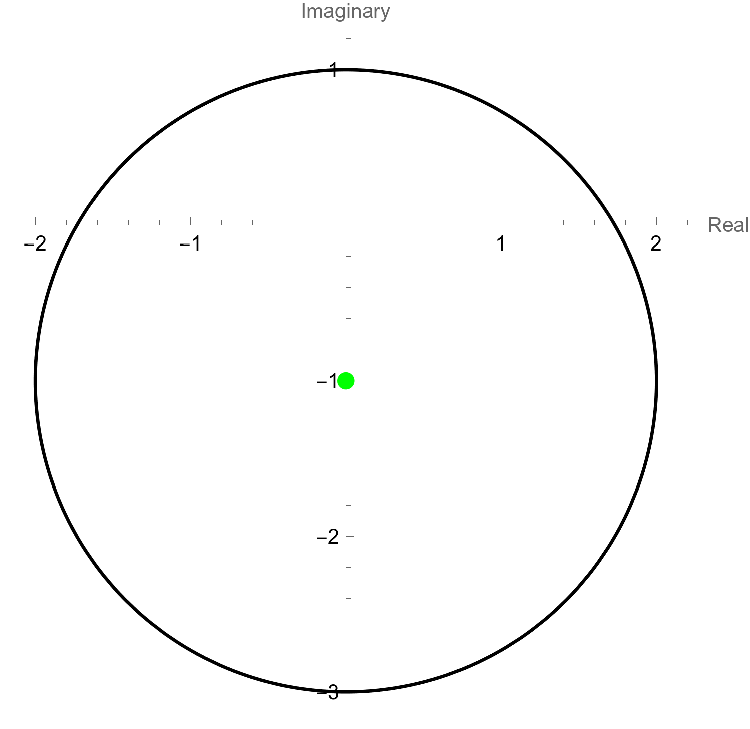
\includegraphics[scale=0.4]{./img/p14-3_b}
	\caption{Vecindad de radio $2$ del punto $-i$.}
\end{figure}


\subsection{Problema 14.4}
\begin{figure}[H]
	\centering
	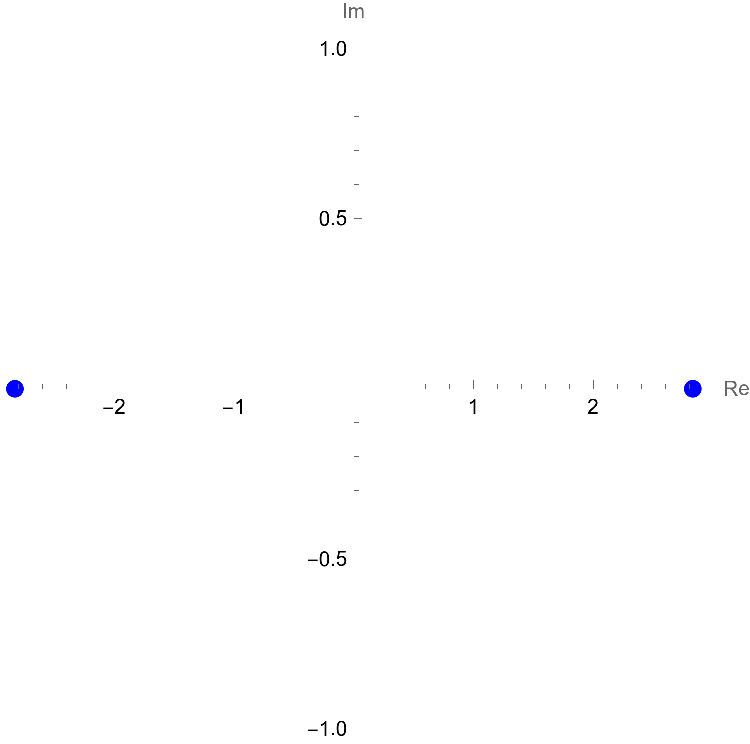
\includegraphics[scale=0.4]{./img/p14-4_a}
	\caption{Soluciones de $z^2 = 8$.}
\end{figure}


\begin{figure}[H]
	\centering
	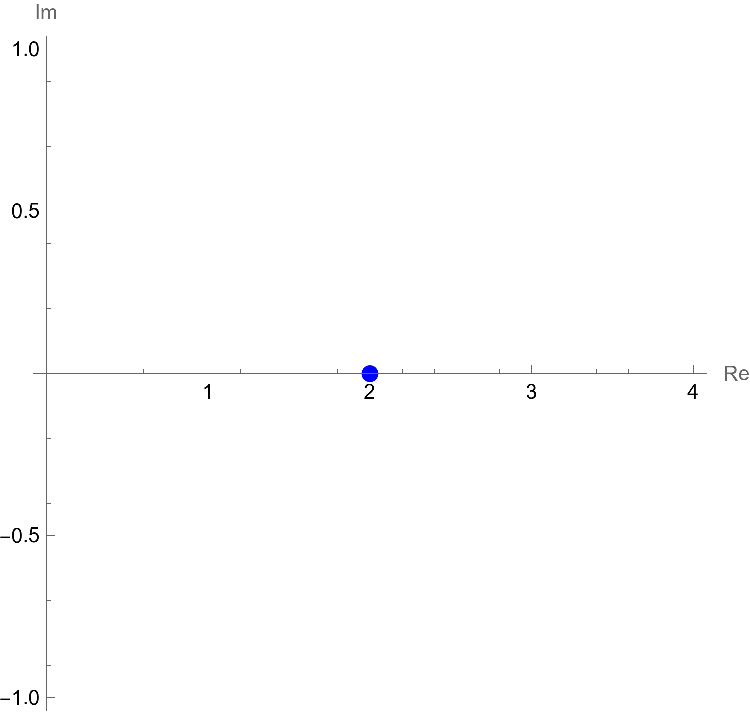
\includegraphics[scale=0.4]{./img/p14-4_b}
	\caption{Soluciones de $z^3 = 8$.}
\end{figure}


\begin{figure}[H]
	\centering
	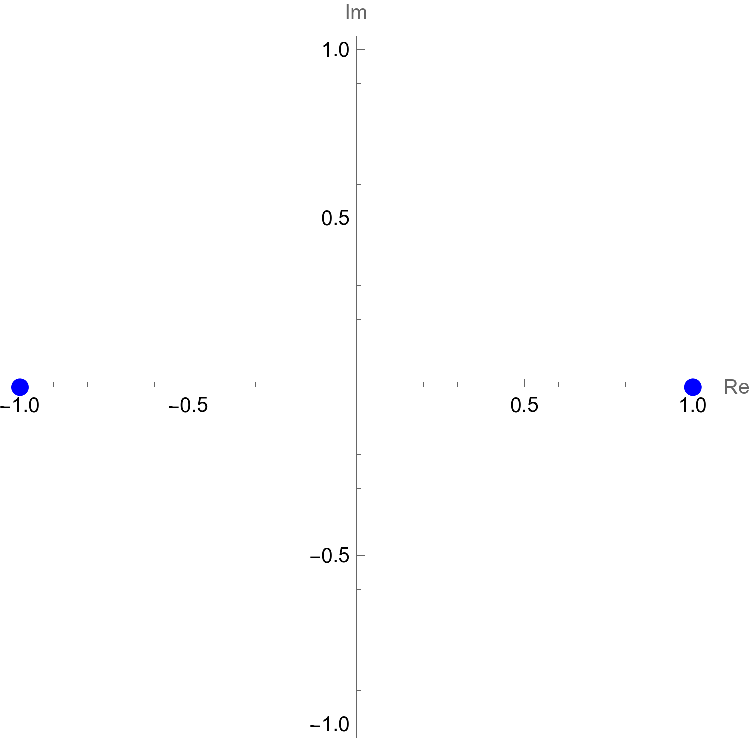
\includegraphics[scale=0.4]{./img/p14-4_c}
	\caption{Soluciones de $z^2 = 1$.}
\end{figure}


\begin{figure}[H]
	\centering
	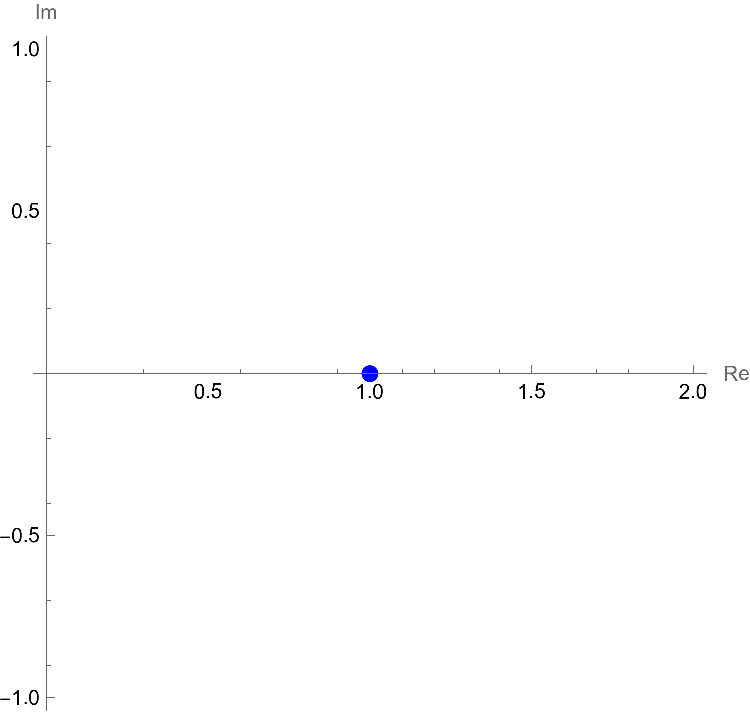
\includegraphics[scale=0.4]{./img/p14-4_d}
	\caption{Soluciones de $z^3 = 1$.}
\end{figure}


\begin{figure}[H]
	\centering
	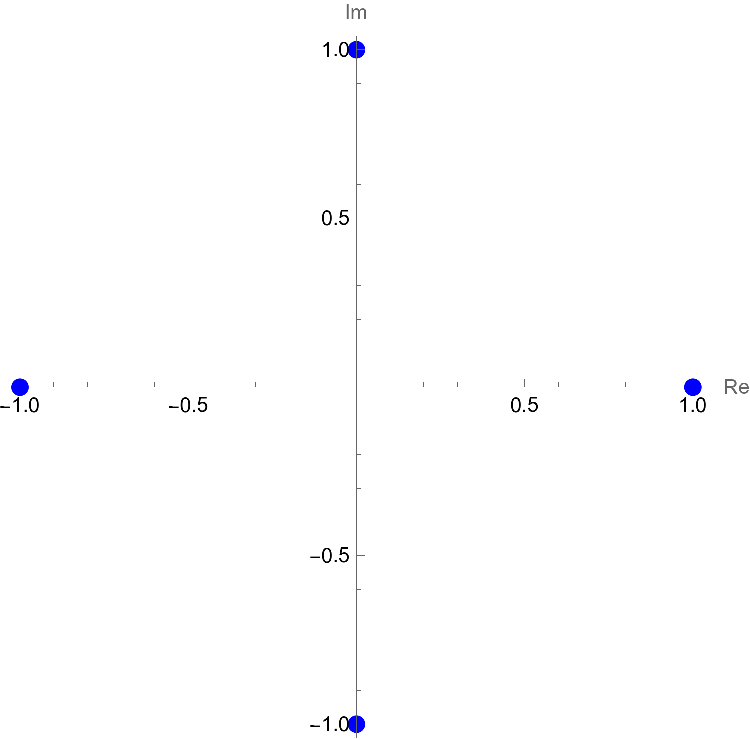
\includegraphics[scale=0.4]{./img/p14-4_e}
	\caption{Soluciones de $z^4 = 1$.}
\end{figure}


\begin{figure}[H]
	\centering
	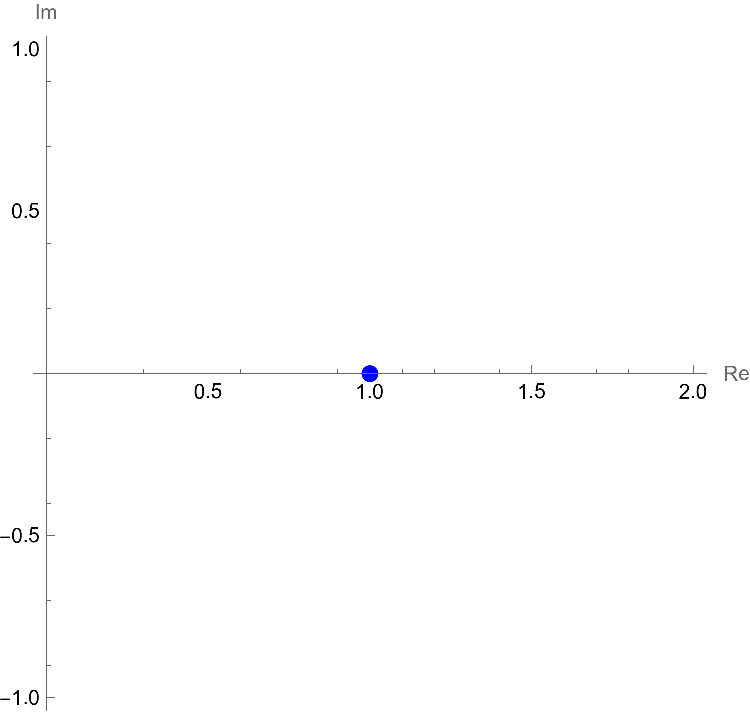
\includegraphics[scale=0.4]{./img/p14-4_f}
	\caption{Soluciones de $z^5 = 1$.}
\end{figure}


\begin{figure}[H]
	\centering
	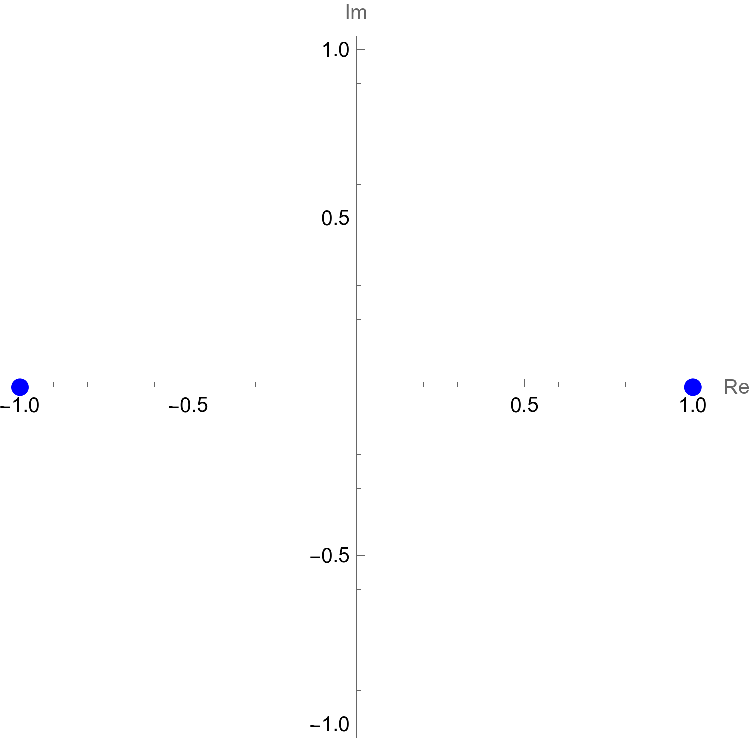
\includegraphics[scale=0.4]{./img/p14-4_g}
	\caption{Soluciones de $z^6 = 1$.}
\end{figure}


\subsection{Problema 14.6}
Regresando a la parte de métrica, se tiene $d(a+bi,c+di) = \sqrt{(c-a)^2 + (d-b)^2}$. 
\begin{itemize}
	\item \textbf{Semidefinido Positivo:} dado que el interior de la raíz es positivo, la función es positiva para todos los $z_1 ,z_2$.
	\item \textbf{Simetría:} Dado que $(x-y)^2 = (y-x)^2$, la función es simétrica.
	\item \textbf{Identidad de los Indesceribles:} Es claramente cierta.
	\item \textbf{Desigualdad Triangular:} Dado que $\sqrt{x} + \sqrt{y} \geq \sqrt{x+y}$, es trivial la desigualdad triangular.
\end{itemize}
Lo que implica que la función $d(a+bi,c+di)$ es una métrica.










\section{Capítulo 15}










%\begin{abstract}
%
%\end{abstract}
%
%\begin{IEEEkeywords}
%
%\end{IEEEkeywords}
%
%\section{Objetivos}
%
%\subsection{General}
%    \begin{enumerate}[1.]
%        \item 
%    \end{enumerate}
%\subsection{Específicos}
%    \begin{enumerate}
%        \item 
%        \item 
%        \item 
%    \end{enumerate}
%%\section{Introducción}
%    
%\section{Marco Teórico}
%    
%    
%\section{Diseño Experimental}
%    \subsection{Materiales a Utilizar}
%        \begin{itemize}
%        \item 
%    \end{itemize}
%
%    \subsection{Procedimientos}
%        \begin{enumerate}
%            \item 
%            \item 
%            \item 
%        \end{enumerate}
%\section{Resultados}
%    
%\section{Conclusiones}
%\begin{enumerate}
%    \item 
%    \item 
%\end{enumerate}
%%\section{Recomendaciones}
%
%\section{Anexos}
%    
%    
%%    \begin{figure}[H]
%%        \centering
%%        \includegraphics[width = 0.5\textwidth]{Imagenes/DiagEstado2.png}
%%        \caption{Diagrama de estados para el semáforo de la calle.}
%%        \label{fig:DiagCalle}
%%    \end{figure}
    
    
\begin{thebibliography}{00}
\bibitem{b1} Holmgren, R. (2000). \textit{A first course in discrete dynamical systems}. Springer Science \& Business Media.
\bibitem{b2} Brown, R. (2018). \textit{A modern introduction to dynamical systems}. Oxford University Press.
\end{thebibliography}

\end{document}


